This chapter describes the technical foundations of the system and how the problems described in section~\ref{sec:problem} have been addressed in Rymd.

% TODO: MUST do concrete descriptions of each module in Rymd here!

%TODO: Motivate choice of AES-CBC-256 (in implementation?)
%Why RSA and not diffie hellman?

\section{Data storage}

Storage of data is, suffice to say, crucial for any file sharing system. Since the data store was to be used by several parts of the application the demands for the module's interface had to be as general as possible, adhering to a standard CRUD\footnote{Create–Read–Update–Delete} interface, including methods for creating, fetching, updating and deleting records in the store.

There are essentially four alternatives for persisting data on the client:

\begin{itemize}
\item LocalStorage
\item IndexedDB
\item WebSQL
\item FileSystem API
\end{itemize}

LocalStorage is included in the HTML5 WebStorage specification \cite{WebStorage:Online}, and is a basic key-value store with a simplistic API. It is supported across all major browsers and has a maximum storage limit of 5 megabytes. The latter was a deal-breaker, since the product would have to support larger files than could possibly fit into that space. LocalStorage further does not support complex structures and indexing, and storing different data types is complex and needs manual serialization and deserialization. Thus this solution was rejected at once.

IndexedDB and WebSQL are both client side databases and more sophisticated storage solutions than LocalStorage. WebSQL is supported by Google Chrome, Apple Safari (desktop and iOS), Opera and Android. The specification is not longer maintained by W3C \cite{WebSQL:Online}, and will probably be deprecated on all browsers in the future. IndexedDB is supported by all major browsers except for Safari (desktop and iOS), and is a Candidate Recommendation by W3C \cite{IndexedDB:Online}. Arbitrary types of data can be stored in the database, such as strings, numbers, Javascript objects, and raw binary data.

The FileSystem API is a collection of methods for reading and writing to a sandboxed filesystem from a browser with client Javascript code. It is a very early standard, and is currently only supported by Google Chrome and Opera, and has the status of Working Draft by W3C \cite{FileSystem:Online}. While FileSystem has good performance for larger files and a well-performing asynchronous API, it lacks support for indexing and search. Mozilla seems to have no plans on implementing FileSystem in Firefox \cite{MozillaFileSystem:Online}.

All of the mentioned technologies are sandboxed: the data is tied to a single origin (\emph{http://test.domain.com} for instance). All future access to the data must come from that domain (this includes the protocol and port number as well). The browsers also limits the maximum allowed storage size – the quota. The quota is different for each storage mechanism, and the browser typically asks the user with a dialog if they want to let the app exceed the quota.

\begin{table}
    \begin{tabular}{|l|l|l|l|l|}
    \hline
                       & IndexedDB & WebSQL & File System & LocalStorage \\ \hline
    Google Chrome 34               & Yes       & Yes    & Yes  & Yes                      \\ \hline
    Mozilla Firefox 29             & Yes       & \cellcolor{red}No  & \cellcolor{red}No   & Yes                        \\ \hline
    Apple Safari 7                & \cellcolor{red}No        & Yes  & \cellcolor{red}No    & Yes                        \\ \hline
    Opera 20                       & Yes       & Yes    & Yes  & Yes                      \\ \hline
    Microsoft Internet Explorer 11 & Yes       & \cellcolor{red}No  & \cellcolor{red}No   & Yes                        \\ \hline
    \end{tabular}
    \caption {Browser support for selected HTML5 APIs at the time of writing}
\end{table}

The conclusion was to use IndexedDB for persisted resource storage. It was chosen because of its support by Google Chrome, Internet Explorer and Firefox, and due to the fact that its actively maintained (while WebSQL is not). Users of the Safari browser will not be able to utilize the product, but in respect to the project's overall direction in regards to experimental technologies, this is negligible.

\section{Peer identity verification}
\label{sec:authorization}
For a truly decentralized system, it is not acceptable to adapt a CA-entered approach. While a Web of Trust is interesting, it might be too cumbersome for users. This issue is addressed in "Zooko's Triangle" (See figure~\ref{fig:zooko}), stating that no system assigning names to participants in a network can have the property that names are secure, decentralized and meaningful at the same time. This conjecture has since been proven false by the design of systems such as the blockchain of the cryptocurrency Namecoin, which effectively acts as a cryptographically secured distrubuted hash table (DHT) with unique keys. Users can reserve a name and assign to it a value of their choice by the cost of a small amount of the Namecoin currency (at the time of this writing 0.01 NMC \cite{Namecoin:2014:Online}, which equals roughly 0.03 USD \cite{CryptoCoinCharts:2014:Online}).

Rymd therefore utilizes a DHT for storage of keys to achieve all of these goals: The distributed nature of cryptocurrencies makes it decentralized; peers can choose their own names (identities), giving meaningful names; the small monetary fee required to register a name makes it both secure and prevents massive name-squatting by malicious third parties.

\begin{figure}[h]
\centering
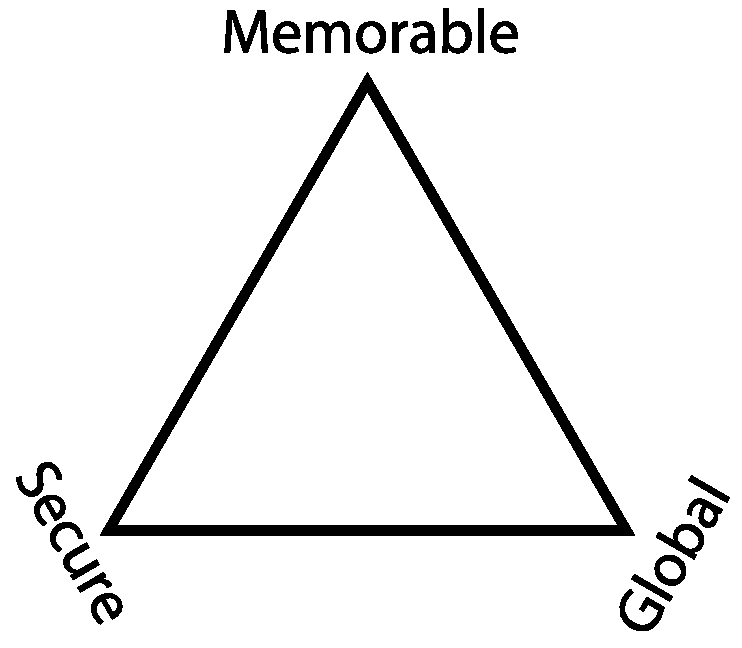
\includegraphics[width=\textwidth,height=0.2\paperheight,keepaspectratio
]{figures/Zooko_s_Triangle}
\caption{Zooko's Triangle, with the edges representing the achievable combinations of features \cite{Zooko:2001:Online}}
\label{fig:zooko}
\end{figure}

%TODO: Draft, references
Once a key distribution scheme has been established, an authentication scheme needs to be determined. There are several schemes for authentication using public-key cryptography. Among these are Otway Rees (not mutual, MITM attack exists), Wide Mouth Frog (depends on timestamps), and Needham-Schroeder. Of the ones surveyed, Needham-Schroeder stood out as simple to implement since it does not utilize symmetric keys or timestamps, while it provides mutual authentication.
%describe needham schroeder

In 1995, Gavin Lowe described a man-in-the-middle attack on the protocol where an adversary that can initiate a session with one party can then pose as that party when communicating with a third party. Schroeder also proposed a fix to this vulnerability, and this amended \emph{Needham-Schroeder-Lowe protocol} presented below is what Rymd utilizes for authentication.

%describe needham schroeder lowe

\section{Decentralization}
Assuming that the system can utilize a DHT such as a cryptocurrency blockchain for storage of the public part of RSA key pairs, the issue of how to interface a web application with the blockchain in a way that allows for verification of identities without putting too much trust in the HTTP/cryptocurrency gateway also needs to be addressed. Additionally, as previously stated, the initial insertion of the key requires monetary resources, and is something that should be solved outside of Rymd. Users can either provide their existing keys and identity to Rymd or let Rymd generate a new pair of keys and manually insert the public part in the DHT of choice.
While the public key can be stored in a DHT, private keys need to be stored securely on each client, preferably without giving client code any direct access to the raw keys.

\section{Creation and transfers of resources}

Full access to a resource implies possession of three things: The encrypted resource data, they cryptographic key used to encrypt said data and the metadata describing the resource. The creation of a new resource goes like this:

% TODO Needs descriptive figure here.

\begin{enumerate}
  \item Metadata is generated. Metadata consists of resource name, author identity, MIME type, a randomly generated GUID, incrementing file version (always $1$ in the case of new resource) and a timestamp.
  \item A resource-specific symmetric cryptographic key is generated. In the default implementation, a 256 bit AES-CBC key is used.
  \item The resource data is encrypted using the resource key.
  \item A resource hash is calculated based on the metadata and encrypted data.
  \item Add the hash to the metadata.
  \item Combine the metadata and the encrypted data to form the internal representation of the resource.
  \item Save the key in a local key store.
\end{enumerate}

To save a resource locally, a user-specific symmetric \emph{master key}, generated at the time of first access, is used to encrypt the metadata before saving it and the encrypted resource data to a local resource store.

Generally, the metadata and the encrypted data are transferred separately - maybe even from separate peers. Therefore the hash is important to verify the integrity of the encrypted data. Resource IDs and hashes could also be communicated via trusted channels outside of Rymd, for example on web pages or via e-mail. Once again, verification of resource integrity and authenticity can be achieved by verifying the hash. It is vital that a secure enough hashing algorithm is used; MD5, which used to be the de-facto standard for generating file checksums, has been proven to be weak and contain vulnerabilities to the extent where checksum collisions are too easy to generate. SHA-1 has for some time been recommended for verification of data integrity, but due to theoretical collision attacks and advances in computational capabilities, the U.S. government currently recommends against SHA-1 for applications that require collision resistance\cite{NIST:2012}. In the default Rymd implementation, the superceding SHA-256 algorithm is used. This gives a strong protection while avoiding the computational overhead of e.g. SHA-512. Note that hashing provides message integrity, but not authentication (establishment of author). This could be established by letting the author of the resource sign the hash with their private key. Peers on the receiving end could then verify the signature using the author's public key. Establishing resource authentication has not been considered a main goal of Rymd and this functionality is therefore not (yet) implemented.

The metadata and resource data are handled separately in Rymd and the communication flow will differ depending on the implementing application. Generally, the metadata will be shared with trusted peers to allow them to decrypt the resource. The encrypted resource can be shared freely since possession of the key is required to make anything useful from it. This way untrusted peers could help facilitate transfers of resources in distributed systems. In the example implementation Shuttle, file sharing is initiated from the sharing end. Consider the case when Bob wishes to share a resource with Alice (assuming both Alice and Bob are already connected to the network):
\begin{enumerate}
  \item Bob requests Alice's public key and endpoint ID's from the DHT.
  \item Bob initiates a connection with Alice and they are mutually authenticated. This process is described below in~\ref{sec:authorization}.
  \item Bob sends the metadata and key for the resource to Alice.
  \item Alice creates a new resource like described above, but without the encrypted data, and saves it to her data store.
  \item Alice requests the resource data from Bob.
  \item Bob sends the encrypted resource data to Alice.
  \item Alice adds the encrypted data to the resource and saves it to the data store.
  \item When Alice wants to access the resource, she decrypts it.
\end{enumerate}

\section{Modules in Rymd}

% TODO Robin: Describe our concrete modules better here. This section *has* to describe how
% *we* used modularity in our project.
